%%%%%%%%%%%%%%%%%%%%%%%%%%%%%%%%%%%%%%%%%
% Beamer Presentation
% LaTeX Template
% Version 1.0 (10/11/12)
%
% This template has been downloaded from:
% http://www.LaTeXTemplates.com
%
% License:
% CC BY-NC-SA 3.0 (http://creativecommons.org/licenses/by-nc-sa/3.0/)
%
%%%%%%%%%%%%%%%%%%%%%%%%%%%%%%%%%%%%%%%%%

%----------------------------------------------------------------------------------------
%	PACKAGES AND THEMES
%----------------------------------------------------------------------------------------

\documentclass{beamer}

\usepackage[utf8]{inputenc}
\usepackage[T1]{fontenc}

\mode<presentation> {

% The Beamer class comes with a number of default slide themes
% which change the colors and layouts of slides. Below this is a list
% of all the themes, uncomment each in turn to see what they look like.

%\usetheme{default}
%\usetheme{AnnArbor}
%\usetheme{Antibes}
%\usetheme{Bergen}
%\usetheme{Berkeley}
%\usetheme{Berlin}
%\usetheme{Boadilla}
%\usetheme{CambridgeUS}
%\usetheme{Copenhagen}
%\usetheme{Darmstadt}
%\usetheme{Dresden}
%\usetheme{Frankfurt}
%\usetheme{Goettingen}
%\usetheme{Hannover}
%\usetheme{Ilmenau}
%\usetheme{JuanLesPins}
%\usetheme{Luebeck}
\usetheme{Madrid}
%\usetheme{Malmoe}
%\usetheme{Marburg}
%\usetheme{Montpellier}
%\usetheme{PaloAlto}
%\usetheme{Pittsburgh}
%\usetheme{Rochester}
%\usetheme{Singapore}
%\usetheme{Szeged}
%\usetheme{Warsaw}

% As well as themes, the Beamer class has a number of color themes
% for any slide theme. Uncomment each of these in turn to see how it
% changes the colors of your current slide theme.

%\usecolortheme{albatross}
%\usecolortheme{beaver}
%\usecolortheme{beetle}
%\usecolortheme{crane}
%\usecolortheme{dolphin}
%\usecolortheme{dove}
%\usecolortheme{fly}
%\usecolortheme{lily}
%\usecolortheme{orchid}
%\usecolortheme{rose}
%\usecolortheme{seagull}
\usecolortheme{seahorse}
%\usecolortheme{whale}
%\usecolortheme{wolverine}

%\setbeamertemplate{footline} % To remove the footer line in all slides uncomment this line
%\setbeamertemplate{footline}[page number] % To replace the footer line in all slides with a simple slide count uncomment this line

%\setbeamertemplate{navigation symbols}{} % To remove the navigation symbols from the bottom of all slides uncomment this line
}

\usepackage{graphicx} % Allows including images
\usepackage{booktabs} % Allows the use of \toprule, \midrule and \bottomrule in tables
\graphicspath{ {images/} }

%----------------------------------------------------------------------------------------
%	TITLE PAGE
%----------------------------------------------------------------------------------------

\title[User Namespaces]{Using Containers Without Risking Your *aas (Canonical) } % The short title appears at the bottom of every slide, the full title is only on the title page

\author{Serge Hallyn, Scott Moser} % Your name
\institute[Canonical] % Your institution as it will appear on the bottom of every slide, may be shorthand to save space
{
Canonical, Inc \\ % Your institution for the title page
\medskip
\textit{serge.hallyn@ubuntu.com, scott.moser@canonical.com} % Your email address
}
\date{\today} % Date, can be changed to a custom date

\begin{document}

\begin{frame}
\titlepage % Print the title page as the first slide
\end{frame}

\begin{frame}
\frametitle{Overview} % Table of contents slide, comment this block out to remove it
\tableofcontents % Throughout your presentation, if you choose to use \section{} and \subsection{} commands, these will automatically be printed on this slide as an overview of your presentation
\end{frame}

%----------------------------------------------------------------------------------------
%	PRESENTATION SLIDES
%----------------------------------------------------------------------------------------

\section{Quick Introduction to Containers}
\begin{frame}
   \frametitle{Linux Containers?}
   \begin{itemize}
      \item operating system-level virtualization method for running multiple isolated Linux systems (containers) on a single control host.
      \item "chroot on steroids"
      \item "it's like bsd jails" (or solaris zones)
      \item from the inside looks like a vm
      \item from the outside looks like processes
    \end{itemize}
\end{frame}

%\begin{frame}
%   \frametitle{Linux Kernel Containment features}
%   \begin{itemize}
%      \item Kernel namespaces (ipc, uts, mount, pid, network and user). Absent: sys, proc
%      \item Apparmor and SELinux profiles
%      \item Kernel capabilities (sys\_boot, sys\_chroot, sys\_module, net\_bind\_service, sys\_mknod)
%      \item Control groups / cgroups (limit memory, accounting/throttling, limit device node operations)
%      \item Chroots (using pivot\_root)
%      \item Seccomp policies
%   \end{itemize}
%\end{frame}

%------------------------------------------------
\section{State of Containers Prior to User namespaces} % Sections can be created in order to organize your presentation into discrete blocks, all sections and subsections are automatically printed in the table of contents as an overview of the talk
\begin{frame}
\frametitle{Containers prior to user namespaces}
\textbf{Namespaces}
\begin{itemize}
\item $id \rightarrow resource$ mapping
	\begin{itemize}
	\item Prevent resource access by not providing a handle
	\item i.e. pid 1 is not global init
	\item {\tt /etc/shadow} not accessible
	\end{itemize}
\item Many leaks ({\tt /proc/pid/fd/N}
\end{itemize}

\textbf{Control groups}
\begin{enumerate}
\item Resource limits and accounting
\item Limit device access
\item If root, re-mount cgroups and change/escape limits.
\end{enumerate}

\vspace{.25in}

\textbf{Capabilities bounding set}
\begin{enumerate}
\item Limit privs of root in container
\item Root still owns most host files
\item {\tiny http://www.sevagas.com/IMG/pdf/exploiting\_capabilities\_the\_dark\_side.pdf}
\item Prevents useful things like tmpfs mounts
\end{enumerate}
\end{frame}

\begin{frame}
\textbf{LSMs}
\begin{enumerate}
\item Paper over the (huge) remaining holes
\item i.e. prevent {\tt /proc/sys/*} writing, etc
\item "Safe from accidental damage by container root"
\item People always want unsafe exceptions
\item Lack of policy nesting limits use {\em in} containers
\end{enumerate}

\vspace{0.25in}

\textbf{Seccomp}
\begin{enumerate}
\item Prevent use of some syscalls
\item Reduce exposed kernel surface
\item Hard to do generally
\end{enumerate}
\end{frame}

\section{User namespaces}
\begin{frame}
\begin{enumerate}
\item Nevertheless
	\begin{enumerate}
	\item Root in container is still root on host
	\item Any leak = game over
	\item Answer: "Wait for user namespaces"
	\end{enumerate}
\end{enumerate}
\end{frame}

\section{Graphical Demo}
\begin{frame}
Demo Time [sort of].
\begin{enumerate}
   \item Ubuntu 14.10 instance with hostname 'lxc-host'.
   \item 2 users (elsa, anna) are each configured to run lxc unprivileged.
   \item 'showinfo': simple shell filter to 'find' or 'ps' or 'grep'.
   \item 'mywait': Very Exciting. Run it, it prints its pid, uid, gid.  Then creates a file named 'sleeper-user@hostname' and sleeps forever. copied into each container's /usr/local/bin.
\end{enumerate}
\end{frame}

\begin{frame}
Host Processes / Users.
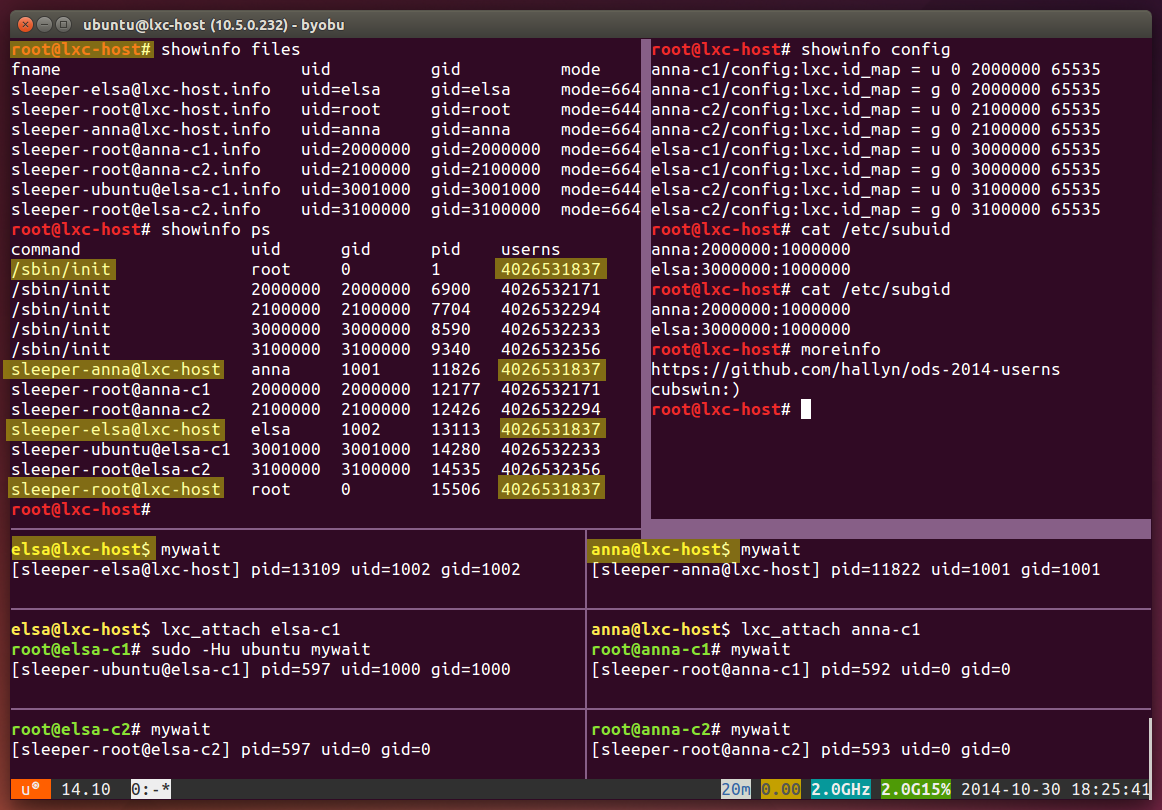
\includegraphics[width=\textwidth]{screen-host-info.png}
%Note:
%  - Multiuser system /sbin/init has pid1.
%  - the userns output of 'ps' shows a uniqiue inode number for each
%    namespace.  The highlighted processes are in the same user namespace.
%  - elsa and anna are both running 'mywait' as unpriviledged users
%    in the top level user namespace.
\end{frame}

\begin{frame}
LXC Containers and Configuration
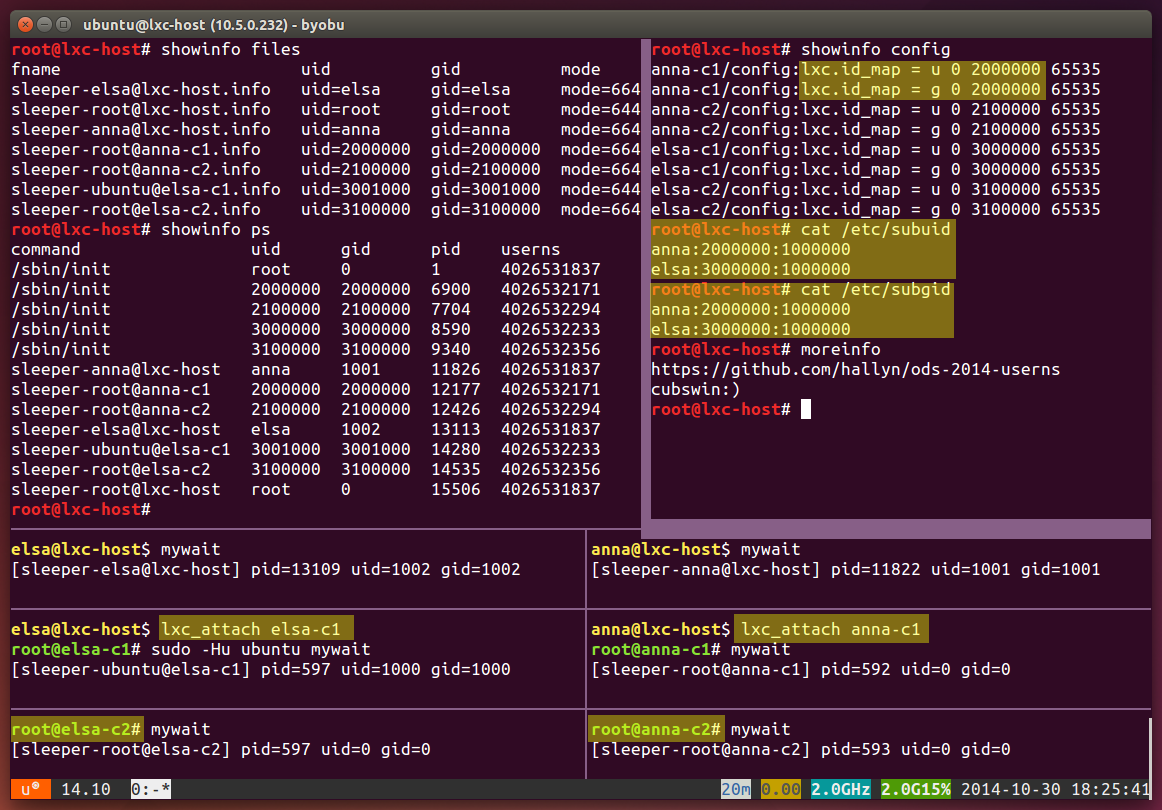
\includegraphics[width=\textwidth]{screen-lxc-config.png}
%  - anna and elsa are given 1 million "subuid" and "subgid" each
%  - fields there say: <user>:start:count
%  - typical linux system allocates 'nobody' to 65535. means without
%    customization, easist solution is to just give 65535
%    thats less than ideal, though as you can only have 65535 of those.
%  - lxc config allows you to map all or a portion of those to a container
\end{frame}

\begin{frame}
Anna's containers: \textbf{anna-c1}, anna-c2
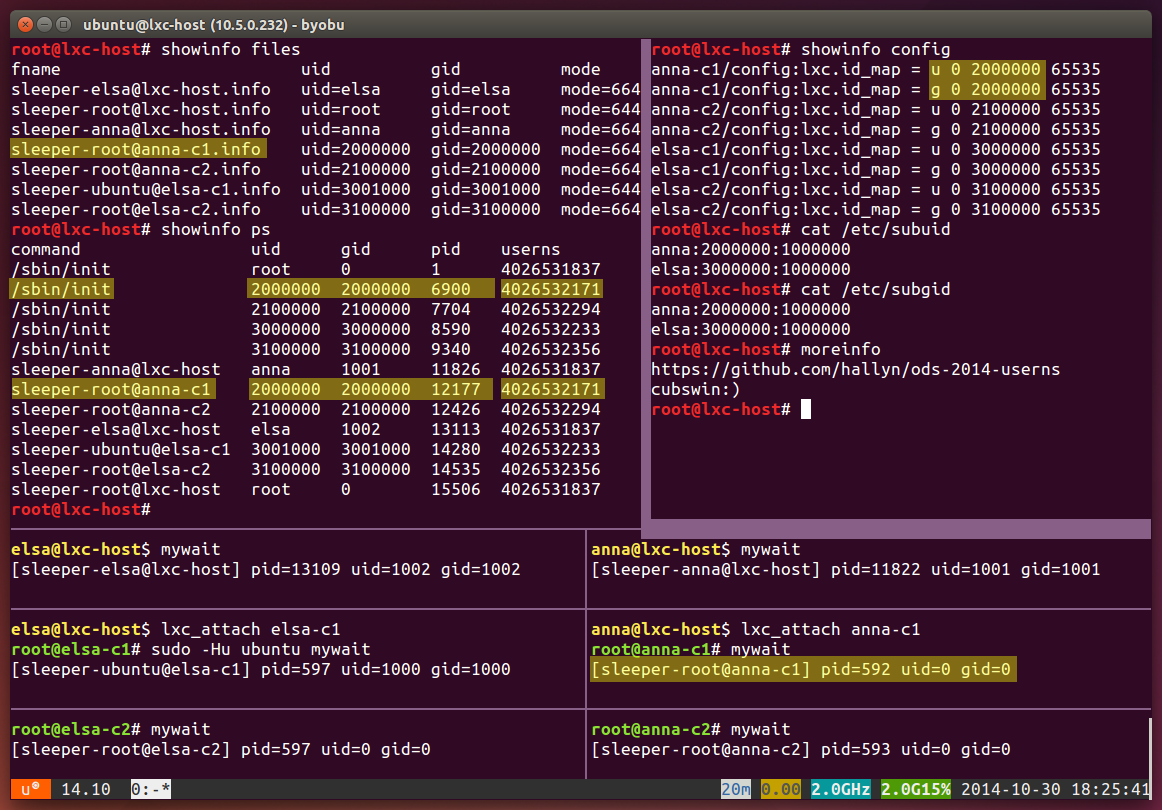
\includegraphics[width=\textwidth]{screen-anna-c1.png}
% Note:
%  - inside container anna-c1, '/sbin/init' believes itself to be
%    pid 1, but from outside it is 6900.
%  - note uid/gid of /sbin/init and 'sleeper-anna-c1' are 2000000
\end{frame}

\begin{frame}
Anna's containers: anna-c1, \textbf{anna-c2}
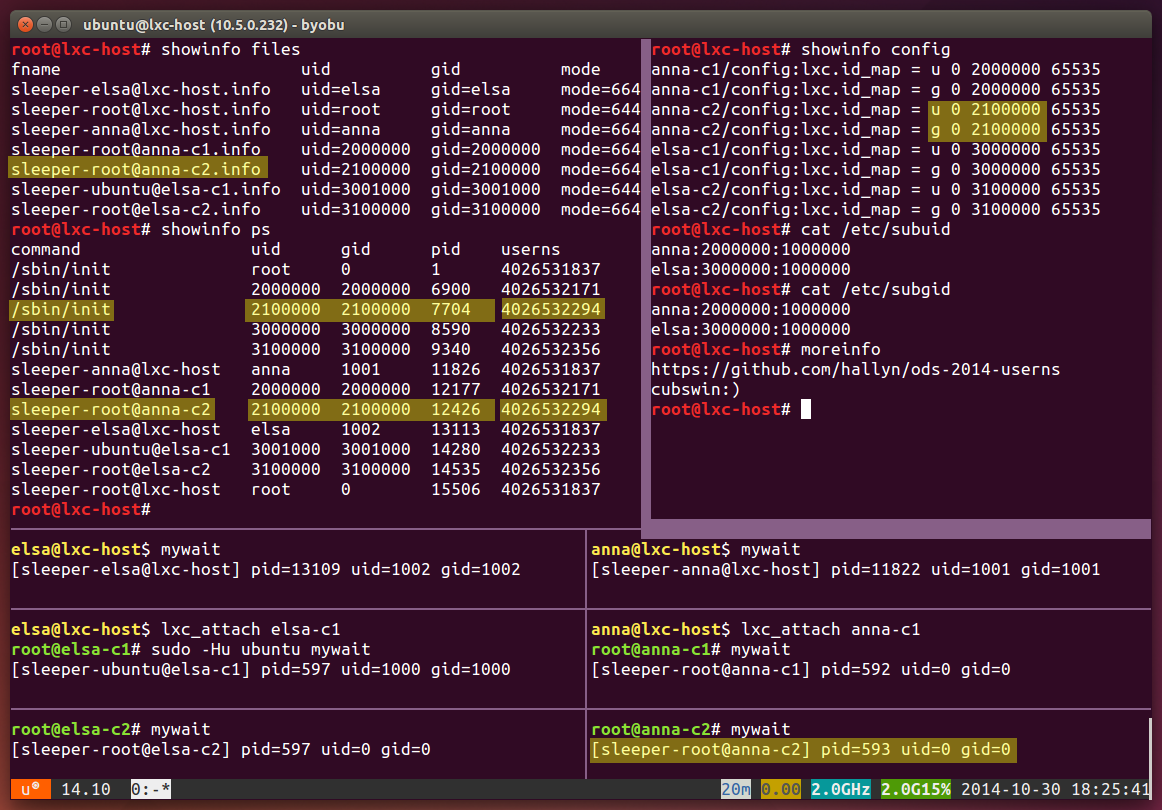
\includegraphics[width=\textwidth]{screen-anna-c2.png}
%Note:
%  - anna's second container is given a different id_map range.
%    2,100,000 rather than 2,000,000
%  - container escape from anna-c2 leaves user 2100000, unable to read files
%    owned by anna (1001) or even anna-c1. (Unless they're world readable).
\end{frame}

\begin{frame}
Elsa's Containers: \textbf{elsa-c1}, elsa-c2
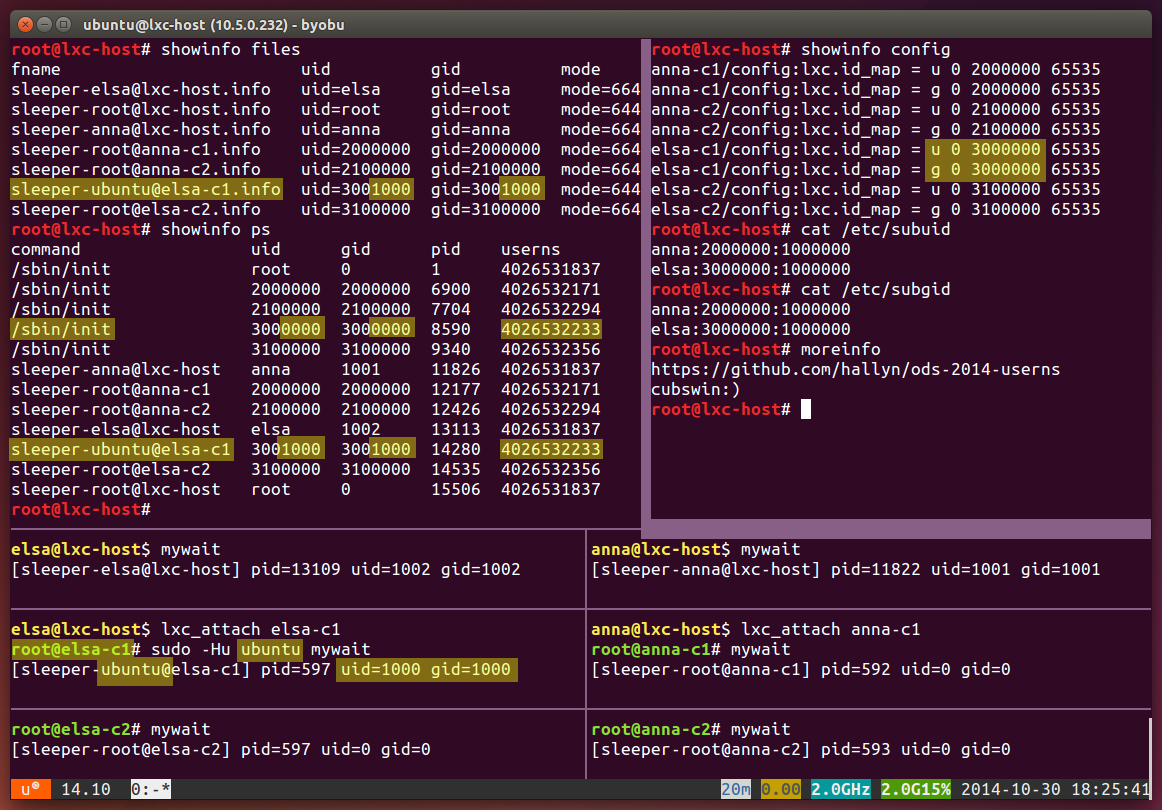
\includegraphics[width=\textwidth]{screen-elsa-c1.png}
%Note:
%  - elsa's second container runs 'mywait' as non-root
%  - note that /sbin/init and sleeper-ubuntu processes have different uid/gid
%  - inside container uid/gid is allocated just as it is on the host
%    even supporting sub-namepaces.
\end{frame}

\begin{frame}
Elsa's Containers: elsa-c1, \textbf{elsa-c2}
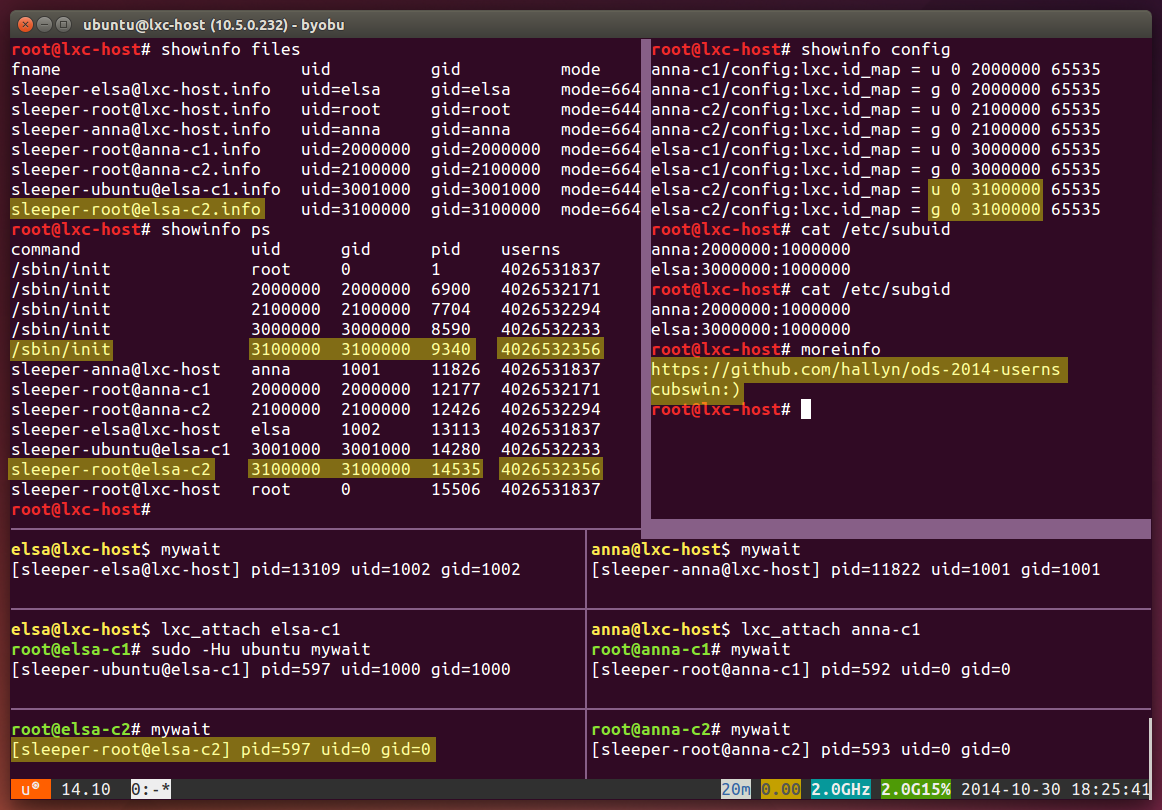
\includegraphics[width=\textwidth]{screen-elsa-c2.png}
%Note:
%  - elsa-c1 has same pid as elsa-c2's sleeper when viewed inside.
%    this is random(ish) coincidence.
\end{frame}

\begin{frame}[fragile]
\frametitle{User namespaces}
\textbf{Goals}
\begin{enumerate}
\item Uid separation
	\begin{enumerate}
	\item c1.500 != c2.500
	\item Separate access controls (kill, open, etc)
	\item Separate accounting, limits
	\end{enumerate}
\item Container root privileged over container
	\begin{enumerate}
	\item uids
	\item network
	\item etc
	\end{enumerate}
\item Container root has no privilege outside of container
	\begin{enumerate}
	\item Root in container as safe as unpriv user on host
	\item Safe for use by untrusted users
	\end{enumerate}
\item Able to be nested
\end{enumerate}
\end{frame}

\begin{frame}[fragile]
\textbf{User namespace design}
\begin{enumerate}
\item By Eric Biederman
\item Uids map 1-1 to kuids
	\begin{enumerate}
	\item Translated at kernel-user boundary
	\item Default mapping 0-4294967295:0-4294967295
	\item Unmapped userids show up as -1, has `o' perms
	\item Unpriv user can only map own host uid
	\end{enumerate}
\item Other namespaces owned by a user ns
	\begin{enumerate}
	\item Root in ns has full privilege over what it owns
	\end{enumerate}
\end{enumerate}
\end{frame}

\begin{frame}
\textbf{Uid delegation}
\begin{enumerate}
\item Root delegates {\em subuids} to users
	\begin{enumerate}
	\item {\tt /etc/subuid} and {\tt /etc/subgid}: \
serge:100000:65536
	\item Set using {\tt usermod}: \
usermod -v 100000-200000 -w 100000-200000 serge
	\end{enumerate}
\item Setuid-root programs write to {\tt /proc/self/\{ug\}id\_map}
\item Each user may be delegated a set of subuids and subgids
\end{enumerate}
\end{frame}

%------------------------------------------------

\end{document} 
